\documentclass{mediumfoils}
%\usepackage{arev} 
\usepackage{ctable}
\usepackage[display]{texpower}
\usepackage{hyperref}
\raggedright
\usepackage{amsmath}

\usepackage{ctable}
\usepackage{fancyvrb}
\usepackage{multirow}


%\definecolor{darkblue}{rgb}{.5,0,0} % not really
\definecolor{cite}{rgb}{.5,0,0}
\definecolor{pale}{rgb}{.6,.6,.6}

\definecolor{gray}{rgb}{0.7,0.7,0.7}
\definecolor{darkgray}{rgb}{0.5,0.5,0.5}
\definecolor{darkblue}{rgb}{0.000,0.251,0.502}
\definecolor{bloodred}{rgb}{0.502,0.000,0.000}
\definecolor{darkgreen}{rgb}{0.000,0.502,0.0}

\definecolor{other}{rgb}{0,0,.5}
\usepackage{hyperref}
\hypersetup{colorlinks=true, linkcolor=darkblue, citecolor=darkblue, filecolor=darkblue, pagecolor=darkblue, urlcolor=other}

\newcommand{\mkred}[1]{{\color{bloodred}#1}}
\newcommand{\mkblue}[1]{{\color{darkblue}#1}}
\newcommand{\mkgreen}[1]{{\color{darkgreen}#1}}
\newcommand{\mkgrey}[1]{{\color{pale}#1}}



\graphicspath{{/Users/will/Dropbox/pictures/}{/Users/will/Dropbox/talks/2014/isa-toronto/analysis/}{../../projects/io-article/extraction/}{/Users/will/Dropbox/employment/applications/mannheim-prof/talk/}{/Users/will/Dropbox/talks/2012/esrc-oxford/}{/Users/will/Dropbox/teaching/texas/}{/Users/will/Dropbox/talks/2014/mcgill}{/Users/will/Dropbox/teaching/texas/}{/Users/will/Dropbox/}}

\talktitle{3 Positions:\\ Documents in space!}
\author{\textbf{Will Lowe} University of Mannheim
\and
 \textbf{Sven-Oliver Proksch}\\McGill University}

\date{}
\runningfooter{IQMR, June 2015}
\begin{document}

\maketitle

\slide{Menu}

Session 1: Dictionary-based `classical' content analysis and topic models

Session 2: Classification and evaluation

Session 3: 
\ita
\itm Scaling Models
\ita
\itm Scaling models
\itm Dimensionality
\itm Uncertainty
\itm as a visualisation tool
\itz
\itz

\slide{The bag of words}

\begin{center}
\small
\begin{tabular}{rllllllllll}\toprule
        & ahead & am & am & i & like & look &  & \textcolor{gray}{content} \\ \midrule
doc 1  & 1     & 1  & 1  & 2 & 0    & 1    & \ldots & \textcolor{gray}{$\theta_1$} \\
doc 2  & 0     & 0  & 0  & 1 & 1    & 0    & \ldots & \textcolor{gray}{$\theta_2$} \\ \bottomrule
\end{tabular} 
\normalsize
\end{center}
~\\\

For each research problem involving content analysis we need to ask:
\ita
\itm What \textit{structure} $\theta$ has
\itm What \textit{modeling strategy} to take
\itm What the \textit{relationship} is between $\theta$ and the words (i.e. the model)
\itz

\slide{Answers}

1. $\theta$ is a (possibly multidimensional) position

2. We want a generative model of words: indirect approach

~\\
\centerline{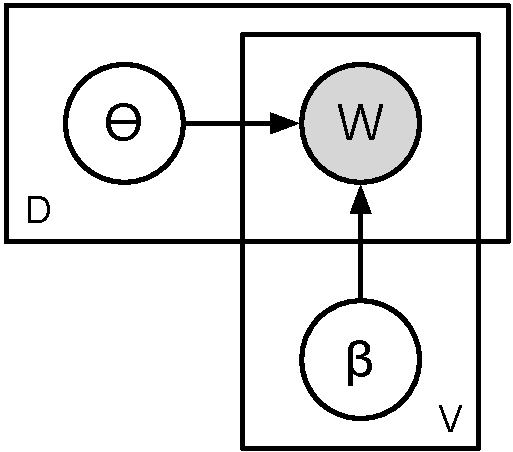
\includegraphics[scale=.6]{scaling-model}}


3. $\theta$ has a proximity (`ideal point') structure connecting document and word positions

\slide{Scaling model}

This class of models puts document \textit{words} (or categories, topics, etc.) in space

\begin{center}
\small
\begin{tabular}{rllllllllll}\toprule
        & ahead & am & i & like & look &  & \textcolor{gray}{content} \\ \midrule
doc 1  & 1     & 1   & 2 & 0    & 1    & \ldots & \textcolor{gray}{$\theta_1$} \\
doc 2  & 0     & 0   & 1 & 1    & 0    & \ldots & \textcolor{gray}{$\theta_2$} \\ 
\vdots \\
&
\textcolor{gray}{$\beta_\text{ahead}$} &
\textcolor{gray}{$\beta_\text{am}$} &
\textcolor{gray}{$\beta_\text{i}$} & 
\textcolor{gray}{$\beta_\text{like}$} & 
\textcolor{gray}{$\beta_\text{look}$}\\
\bottomrule

\end{tabular} 
\normalsize
\end{center}
~\\\


\centerline{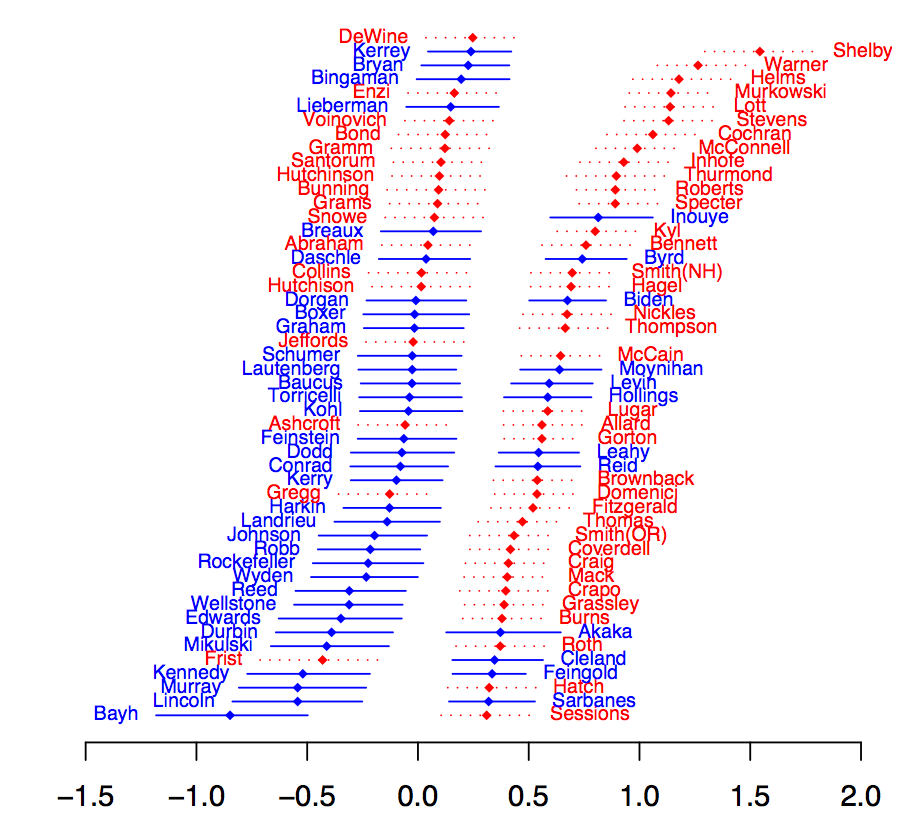
\includegraphics[scale=.45]{senator-ip-monroe-maeda}}


%\slide{Scaling Senate Output}

\slide{German parties 1990-2005}

\centerline{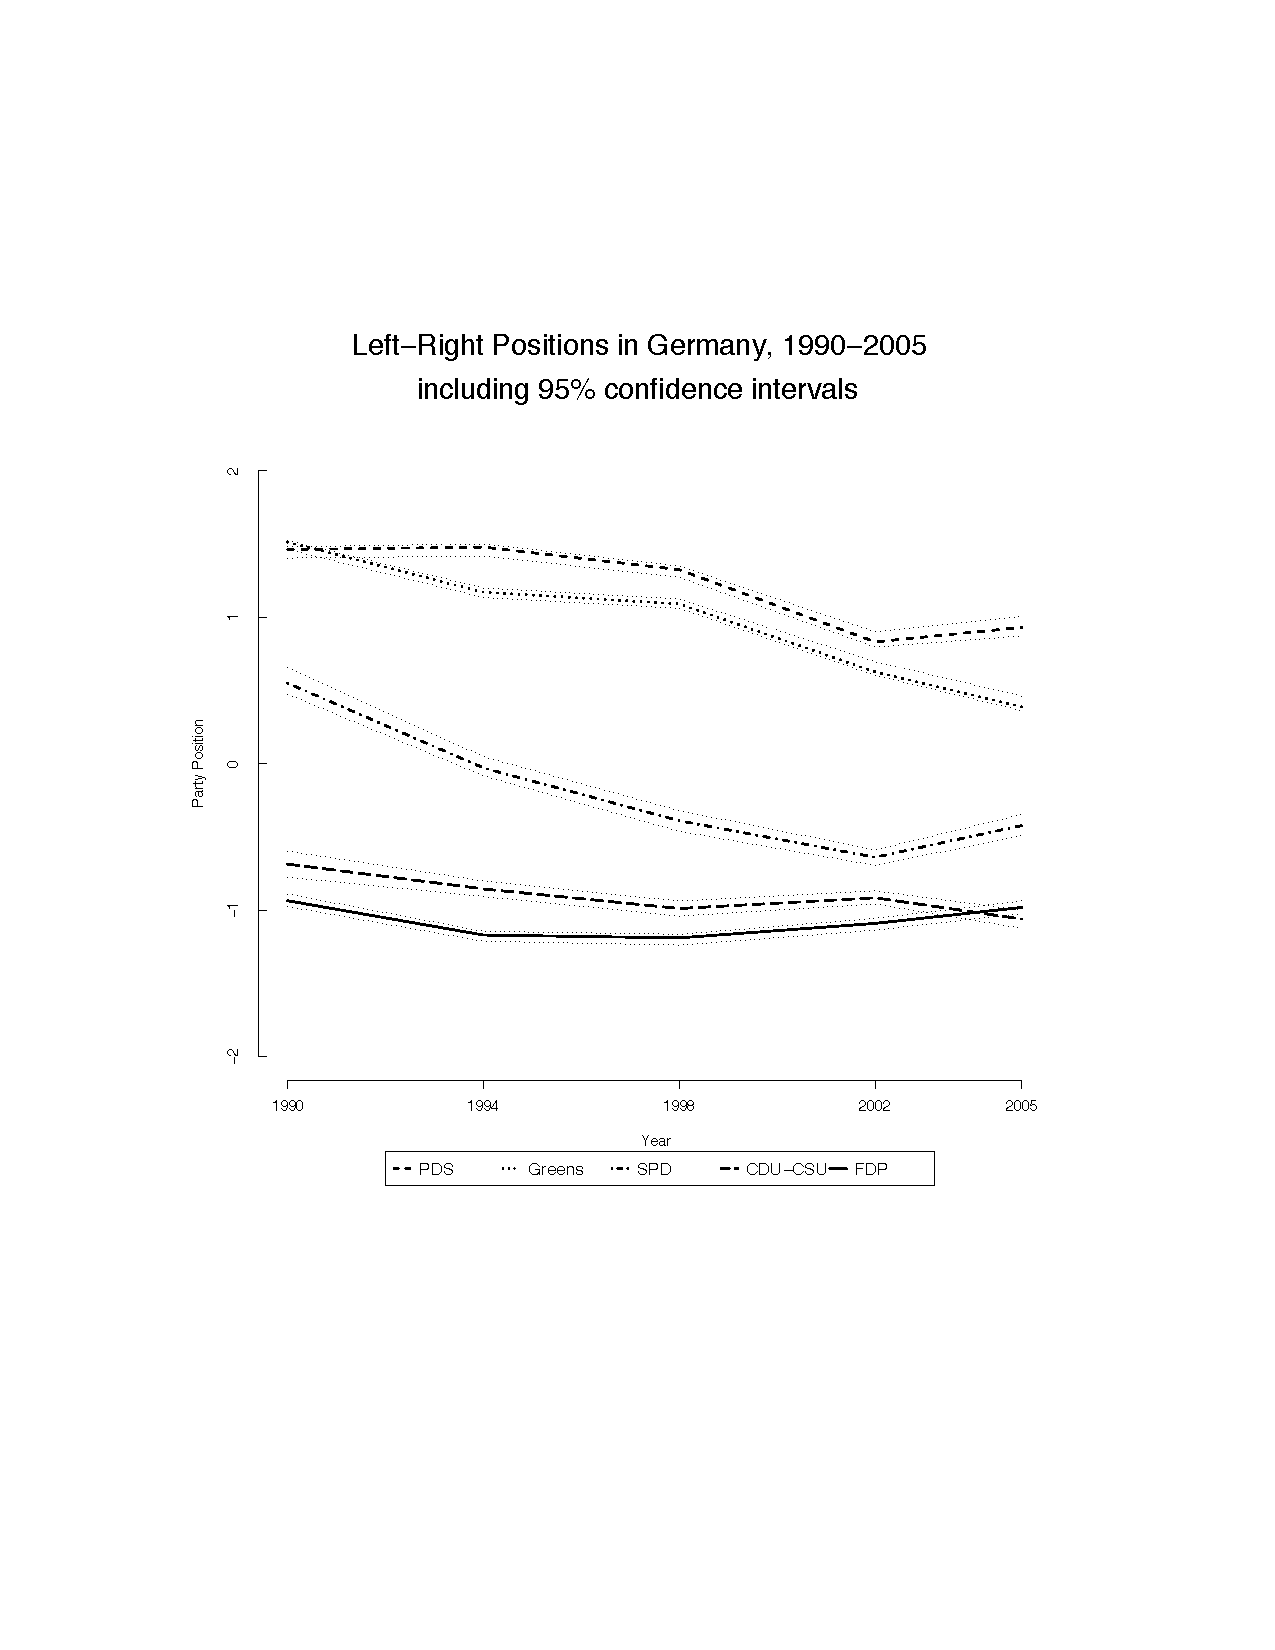
\includegraphics[scale=.85]{poissonscaling}}

\newpage
\centerline{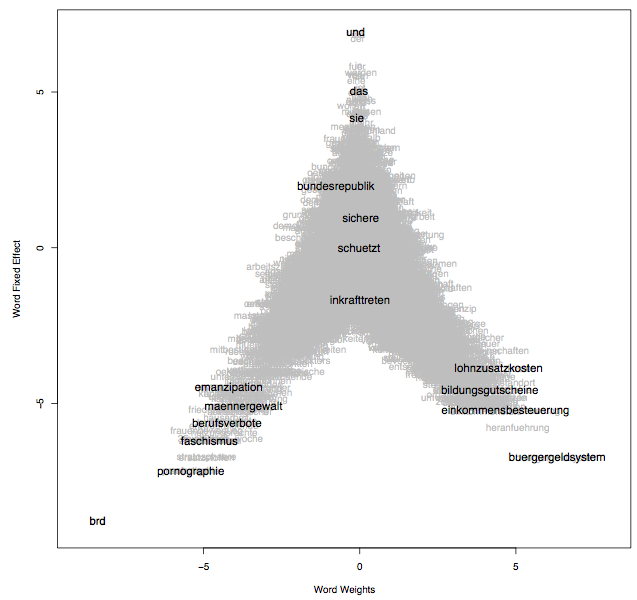
\includegraphics[scale=.75]{sp-informativeness}}


\slide{Structure}

Typically scaling models assume that
\ita
\itm relative word usage is reflective of political ideology
\itm Positions are unidimensional in $W$ 
\itm Positions drive word counts stochastically according to a particular form for $P(W_{j} \mid \theta)$
\itm Bag of words: counts of $W_{j}$ are conditionally independent given $\theta$
\[
P(W_{1}\ldots W_{V}) ~=~ \prod^{V}_{j} P(W_{j} \mid \theta)~ P(\theta)
\] 
\itz 

\slide{Existing Models}

We focus on:
\ita
\itm \textit{Wordfish}: (Slapin and Proksch, 2008)
\itm (Also Laver et al. 2003, Monroe and Maeda, 2004; Beauchamp, 2008; Pennings and Keman, 2002; K\"{o}nig and Luig, 2009, Goodman 1979, etc.)
\itz

%%%%%%%%%%%%%%%%%%%%%%%%%%%%%%%%%%%%%

\slide{Wordfish}

The position word relationship is
\begin{eqnarray*}
W_{ij} &\sim& \text{Poisson}(\mu_{ij})\\
\log \mu_{ij} &=& \psi_{j} + \beta_{j}\theta_{i} +  \alpha_{i} 
\end{eqnarray*}
Each word is a Poisson Process (stochastic component) driven by word and document parameters (the systematic component)


Word parameters:
\ita
\itm $\beta$~~ how fast counts increase or decrease with changes in position
\itm $\psi$~~ how frequent words are irrespective of position
\itz


\slide{Wordfish}

The position word relationship is
\begin{eqnarray*}
W_{ij} &\sim& \text{Poisson}(\mu_{ij})\\
\log \mu_{ij} &=& \psi_{j} + \beta_{j}\theta_{i} +  \alpha_{i}
\end{eqnarray*}
Each word is a Poisson Process driven by word and document parameters

Document parameters:
\ita
\itm $\theta$~~ the position being expressed
\itm $\alpha$~~ a fixed effects for documents controlling for length\ldots
\itz

\slide{An equivalent view}

If document \textit{length} is uninformative about position then we can condition on it. 

In fact Wordfish already does

\begin{eqnarray*}
P(W_{i} \mid \theta_{i}, N) &=& \text{Multinomial}(\boldsymbol{\pi}, N)\\
\log \frac{\pi_{ij}}{\pi_{i1}} &=& \psi^{*}_{j} + \beta^{*}_{j}\theta_{i}
\end{eqnarray*}
where $\psi^{*}_{j} \leftarrow (\psi_{j}-\psi_{1})$, $\beta^{*}_{j} \leftarrow (\beta_{j}-\beta_{1})$ and $\alpha_{i}$ cancels

~\\
Wordfish is secretly a Multinomial Response Model

%\slide{Wordfish}
%
%This matters primarily for predicting the positions of new documents
%\ita
%\itm What $\alpha$ should a new document get?
%\itz
%Also for accurate standard errors
%\ita
%\itm Replace the parametric bootstrap procedure 
%\ita
%\itm ``it may take several days to estimate confidence intervals on a standard desktop computer'' (Wordfish FAQ)
%\itz
%\itm with a cheap asymptotic version
%\itz

\slide{Estimation}

Wordfish models are fit using Conditional Maximum Likelihood (regression without independent variables)
%\ita
%\itm (Not quite an EM algorithm)
%\itz

Iterate:
\ita
\itm Fix document parameters ($\alpha$ and $\theta$) and maximize word parameters ($\beta$ and $\psi$)
\itm Fix new word parameters ($\beta$ and $\psi$) and maximize document parameters ($\alpha$ and $\theta$)
\itz

This can be quite slow depending on the size of your dataset\ldots

%The model is slightly more stable when $\beta$ is regularized 
%\ita
%\itm Equivalent to assuming that $\beta \sim \text{Normal}(0,\sigma^{2})$ a priori
%\itz

%\slide{A Hint of Bayes}

%The iteration embeds an application of Bayes theorem:
%\ita
%\itm In step 2: Assume $P(\theta)$ is constant
%\begin{eqnarray*}
%P(\theta \mid W; \beta, \psi) &~\propto~& P(W \mid \theta; \beta, \psi)~ P(\theta)\\
%\text{Posterior} &~\propto~& \text{Likelihood} ~\times~ \text{Prior}\\
%\theta \Longleftarrow W & & W \longleftarrow \theta,\quad \theta
%\end{eqnarray*}
%Maximize this posterior distribution over $\theta$
%\itz
%~\\
%Note that the Likelihood is really $V$ Likelihoods, one for each word type\ldots


\slide{Identification}
\[\log \mu_{ij} = \psi_{j} + \beta_{j}\theta_{i} +  \alpha_{i}\]

	As is the case with all scaling models (e.g. NOMINATE), the likelihood function is not identified.
		
	  Without fixing some parameters, there are infinite combinations of $\theta$ and $\beta$, which could provide the same likelihood (we would not arrive at a unique solution). 
    

Solution: fix  mean of document positions %$\omega$ 
$\theta$ to 0 and St. Dev. to 1. Set one document fixed effect to 0. Set directionality of scale. This means that you cannot directly compare estimates ACROSS different estimations.




\slide{What about differences across languages?}




 Ideal case: get the exact same political texts in high quality translations

 Estimate Wordfish and compare across different languages

 This is possible: European Parliament speeches (translated into all official languages of the EU)




\slide{What about differences across languages?}

\begin{center}
Positions of National Parties in the European Parliament


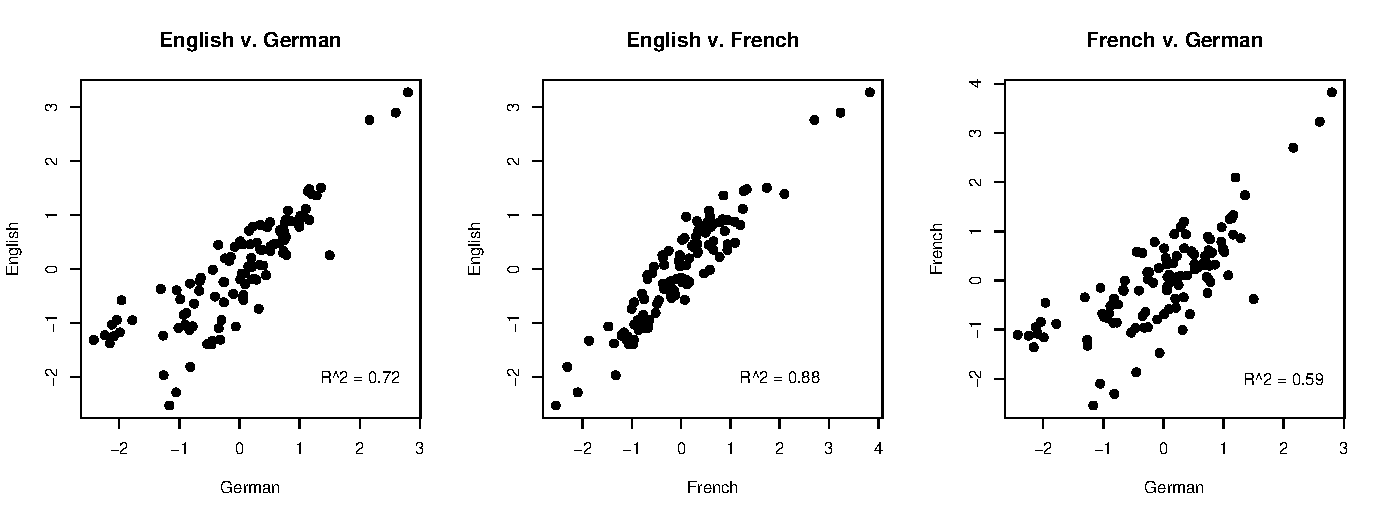
\includegraphics[width=24cm]{scatter_wordfish.pdf}

\end{center}



%\slide{Big Picture: As Measurement}
%
%\begin{center}
%\footnotesize
%\begin{tabular}{ccc}
%\textbf{Distance Measures} & \textbf{Dominance Measures} & \\
% &  & \\
%Parametric Unfolding & Item Response Theory & (Wordfish) \\ 
%$\uparrow$ & $\uparrow$ & \\
%\textsl{approx.} & \textsl{approx.} & \\
%$\mid$ & $\mid$ & \\
%Correspondence Analysis & Factor Analysis & \\
%$\uparrow$ & $\uparrow$ & \\
%\textsl{implements} & \textsl{approx.} & \\
%$\mid$ & $\mid$ & \\
%Reciprocal Averaging & PCA & \\
%$\uparrow$ & & \\
%\textsl{approx.} &  & \\
%$\mid$ & & \\
%Wordscores & & \\
%\end{tabular}
%\normalsize
%\end{center}
%



\slide{Dimension Issues}

What the heck is $\theta$?

How do we know that positions on only one dimension are being expressed in the text?

\slide{Dimension Issues}

What the heck is $\theta$?
\ita
\itm Whatever maximizes the Likelihood\ldots 
\itz
Like all scaling techniques (e.g. NOMINATE), Wordfish is effectively \textit{exploratory} -- you have to figure out what the dimension really is. This is the reason why you need to think about your data before applying the method.


\slide{Dimension Issues}

How do we know that positions on only one dimension are being expressed? How do we get positions on a specific policy issue?

\textit {Force} the assumption to be true by including substantive knowledge about your texts:
\ita
\itm Use only those texts (or sections thereof)  that are guaranteed to be on the same topic and scale them separately 

\itm E.g. speeches from a specific debate or policy sections of manifestos (e.g.  Slapin and Proksch 2008)
\itz
Advantage: Heroic assumptions are (closer to being) true


\slide{Avoiding dimension issues}

Allow for more dimensions!

We need to move to a computationally cheaper model: correspondence analysis (e.g. Greenacre 2007)

For identification, a K-dimensional model has K sets of $\theta$ and K sets of $\beta$ 
\ita
\itm and they'll be orthogonal\ldots
\itz


\slide{Orthogonality?}

But substantively meaningful dimensions do not always line up with the axes of $\theta$\ldots

\newpage

\centerline{\includegraphics[scale=.9]{/Users/will/Desktop/cmp-wrangling/grey-rile.pdf}}

\slide{Dimensions and topic change}

What if the political lexicon changes over time? (it does)
\ita
\itm New issues appear, old issues disappear
\itz

Then scaling algorithms pick up shifts in the policy agenda rather than shifts in party positions. 

\slide{Not avoiding dimensional issues}

\centerline{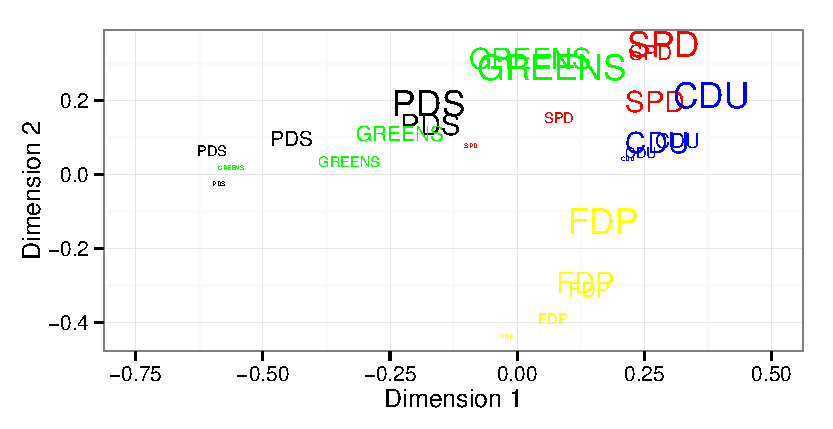
\includegraphics[scale=1]{de-2d}}

\slide{Worst Case Scenario}

\centerline{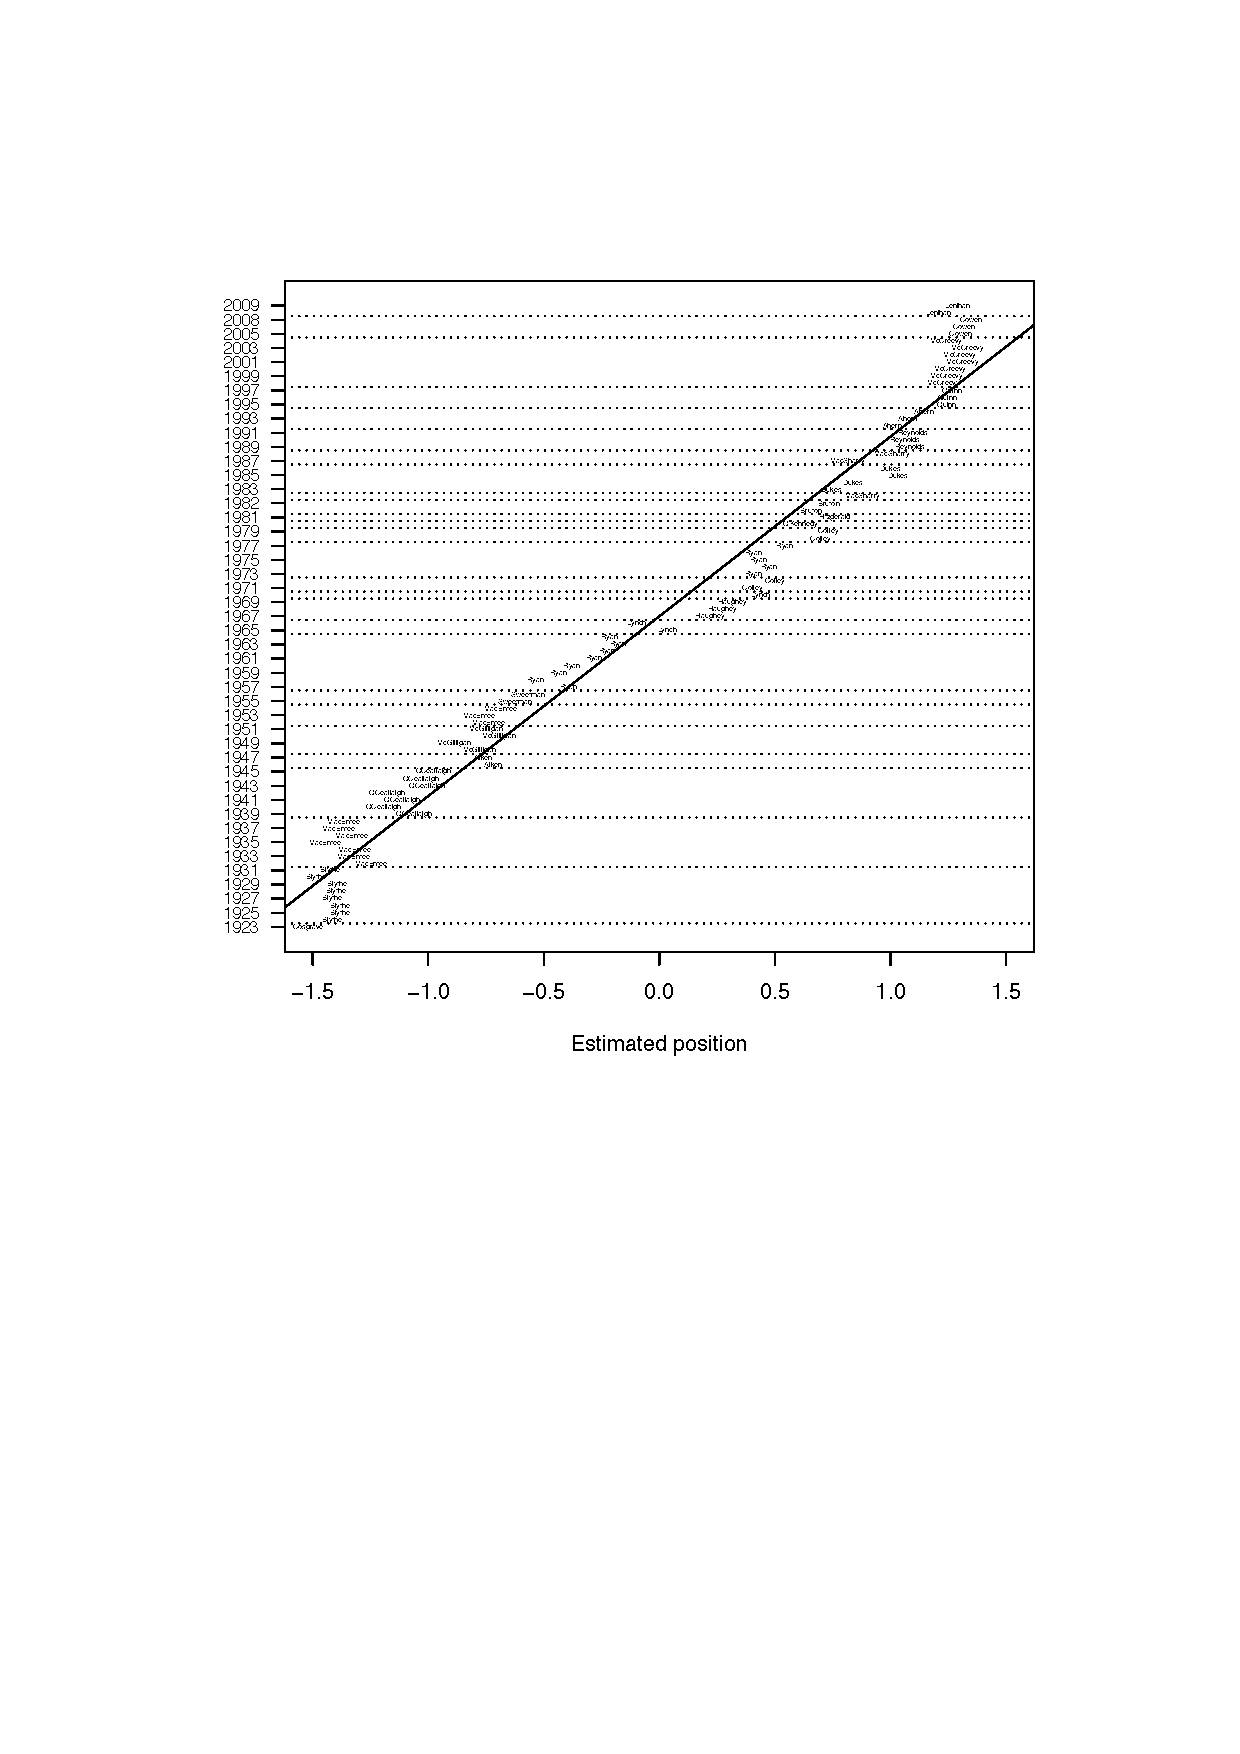
\includegraphics[scale=.9]{pictures/HandMfig2}}

\slide{Dimensions and lexical instability}

\ita
\itm This is a problem with our assumption that all systematic word usage reflects ideology.
\itm When all parties start talking about the `issue' of the day we will distinguish elections, but not parties
\itm We can (try to) get around this by focusing on those words that remain in the political vocabulary across time.
\itz

%: end
%%%%%%%%%%%%%%%%%%%%%%%%


\slide{Validation}

Do these models extract valid positions?
\ita
\itm multiple dimensions, drifting language, and topics
\itm non-dimensional structure
\itm selection bias and party control of the floor
\itz

%\slide{DE parties write about the economy}
%
%\centerline{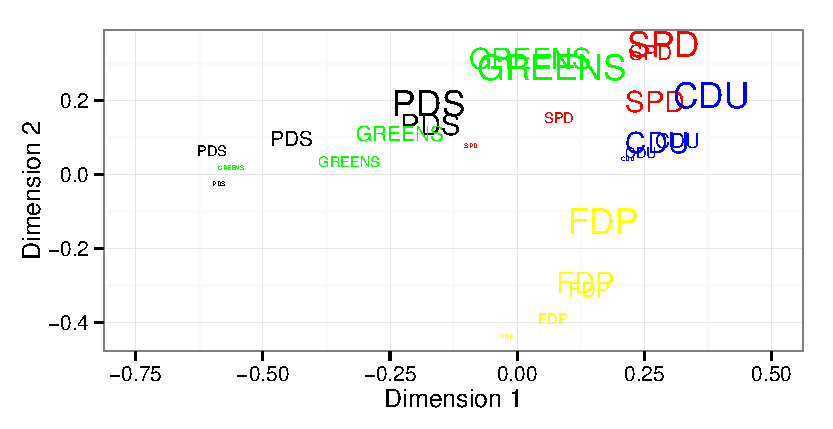
\includegraphics[scale=1.1]{de-2d}}

\slide{Validating positions and uncertainty}

14 speeches from the debate on Ireland's 2010 budget coded by 18 PhD students (LSE and TCD)

{Task}: Identify \textit{speaker positions}, twice
\ita
\itm directly with uncertainty limits \\
by pairwise comparison (and indicate uncertainty)
\itz
\mkgrey{(Lowe \& Benoit 2014)}

\slide{Respondents' positions: direct}

\centerline{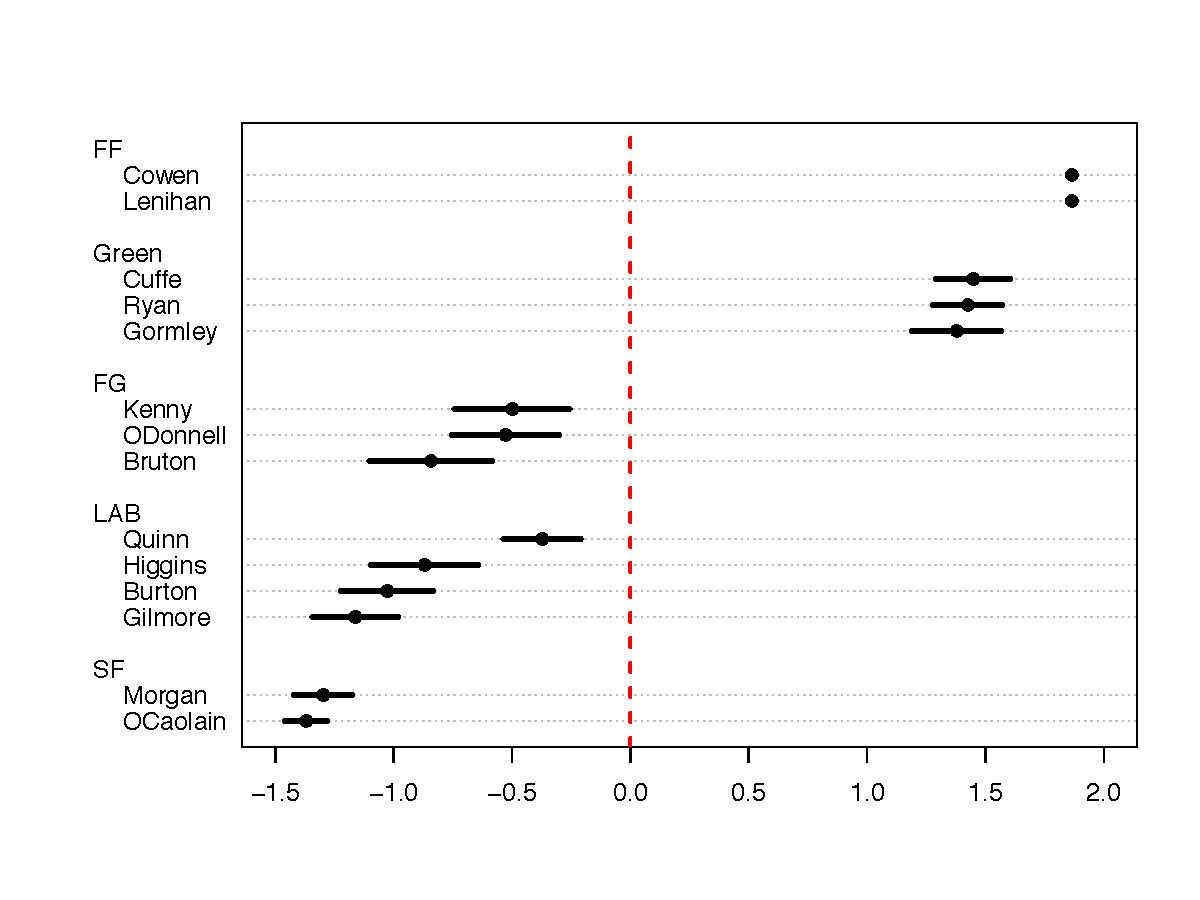
\includegraphics[scale=1]{dotplot_scaled.pdf}}

%\slide{Respondents' positions: pairwise}
%
%\centerline{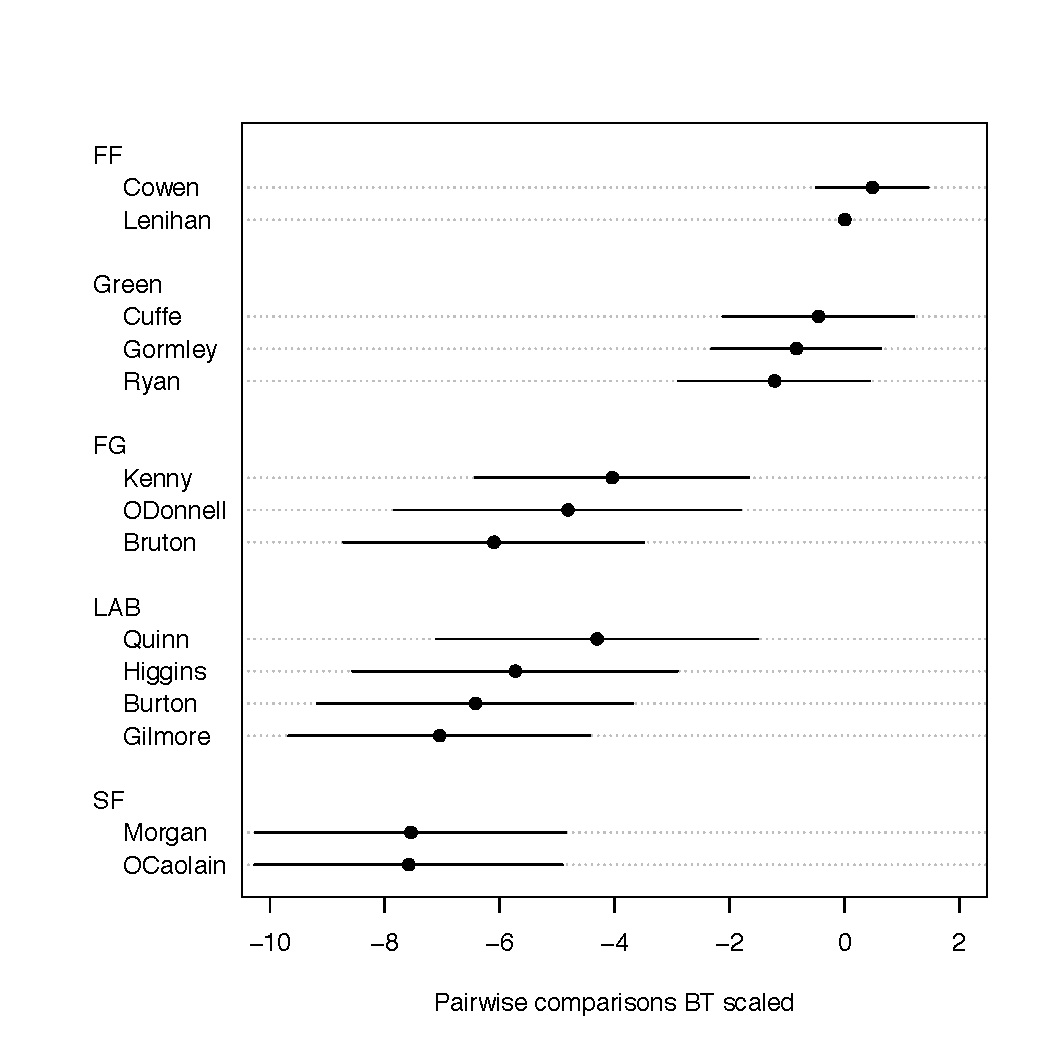
\includegraphics[scale=.7]{less-ugly}}

\slide{Model's positions}

\centerline{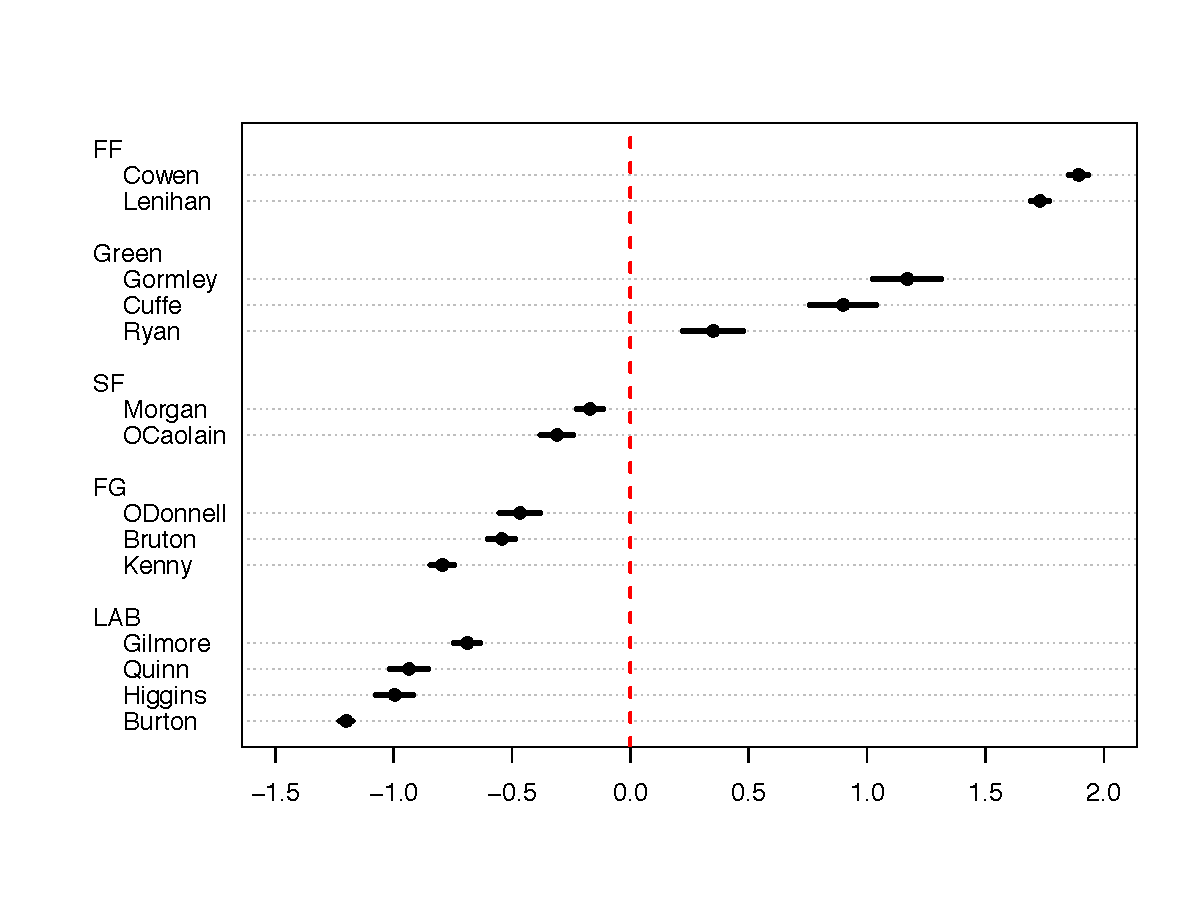
\includegraphics[scale=1]{dotplot_hscaled.pdf}}

\centerline{\includegraphics[scale=.8]{irish-budget-debate}}

\centerline{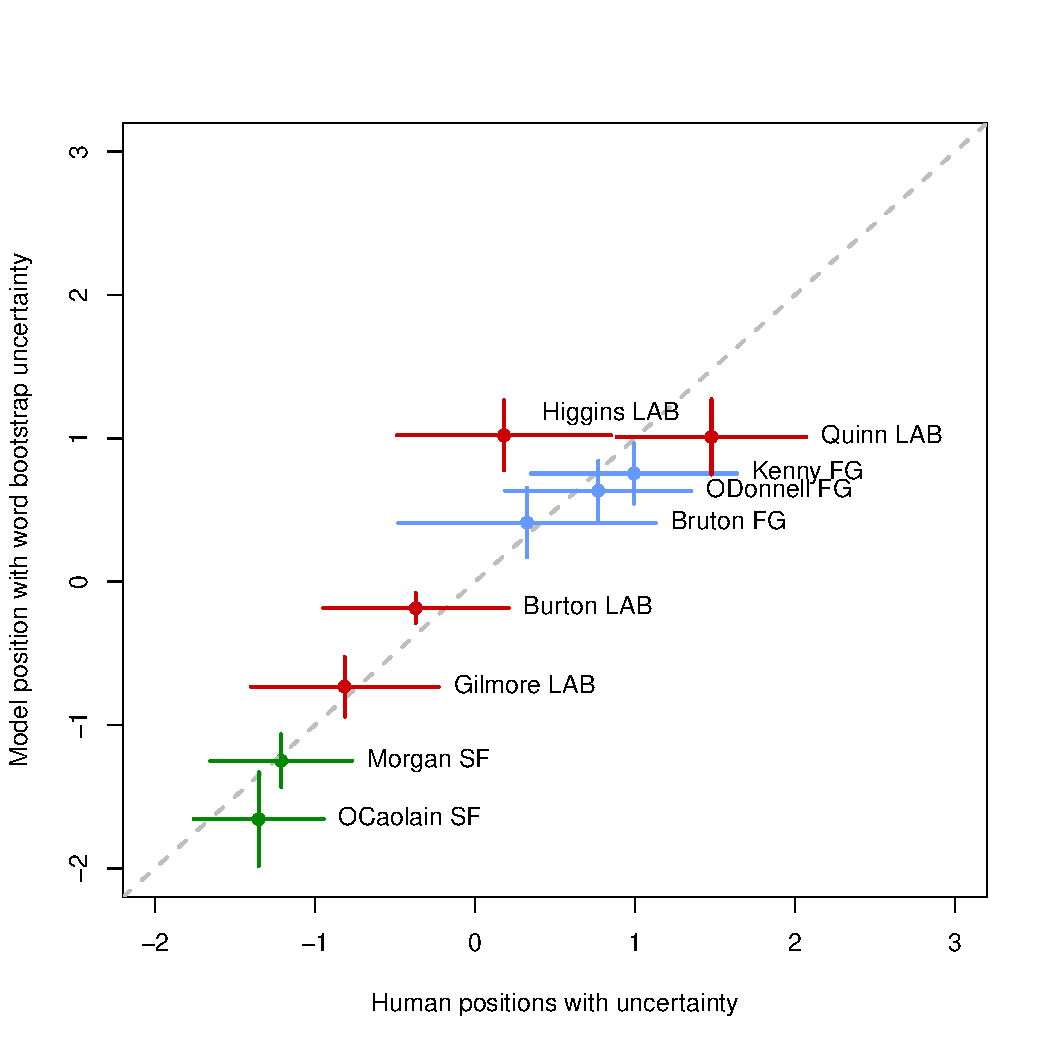
\includegraphics[scale=.9]{opposition_only_comparison}}

\slide{Institutional role}

\centerline{\includegraphics[scale=.9]{mixed-snap}}

~\\
Gormley the Green party member vs Gormley the minister

\slide{Validation: positioning}

These models  
\ita
\itm distinguish \textit{government and opposition} less than coders
\itm correctly \textit{order parties}, {except} for Sinn F\'ein
\itm identify more \textit{variation} in the Green party
\itz
~\\
Individual speaker positions are apparently difficult to assign

%\slide{Validation: uncertainty (five methods)}
%
%Uncertainty measures try to answer the question:
%
%\begin{center}
%\textit{How different could this speech have been?}\\
%(while still expressing the same position)
%\end{center}
%
%\slide{Three ways to be uncertain\\
%(in a model)}
%
%{ML}: assume the model is correct \& \textit{word parameters} are well estimated\\
%{\textcolor{pale}{(Lowe \& Benoit 2010)}}
%
%{Bayes}: assume the model is correct\\
%{\textcolor{pale}{(Monroe \& Maeda 2004, Lo et al. 2011)}}
%
%{Bootstrap}: assume that expected word rate $\mu_{ij}$ is correct\\
%{\textcolor{pale}{(Lowe \& Benoit 2011)}}
%
%\slide{Bootstrapping text}
%
%Resampling `writes' the speeches that could have been given, but weren't\ldots
%\vfill
%\pause
%{parametric}: Resample from the \textit{fitted word counts} and refit
%
%{word}: Resample \textit{individual words} and refit
%
%{sentence}: Resample \textit{natural sentences} and refit
%
%{block}: Resample overlapping length K word sequences
%
%\centerline{\includegraphics[scale=1]{uncertainty_comparison.pdf}}
%
\slide{Conclusions from validation}

Substantively these scaling models induce dimensional structure from patterns of relative emphasis
\ita
\itm This is some, but not all of the structure reported by experts and coders
\itz
They do mostly they recover expert-assigned political positions, but can get fooled by extra-dimensional structure

%They are \textit{over-confident} about position, but this can be \textit{partially corrected}.


\slide{Visualisation}

\begin{center}
But I \textit{don't really care} about the microfoundations\\of political position-taking using text\ldots
\end{center}
\vfill

\slide{An alternative derivation}

Wordfish is a model intermediate in complexity between:
\[
\log \mu_{ij} = \psi_{j} + \alpha_{i}
\]
and
\[
\log \mu_{ij} = \psi_{j} + \alpha_{i} + \eta_{ij} 
\]
by projecting the variation in $\eta_{ij}$ into a lower dimensional space
\[
\eta_{ij} \approx \beta_{j}\theta_{i}   
\]



%: alteder

\slide{Visualising relative emphasis}

6000 manually-coded Tweets from \texttt{\#OccupyWallStreet}, \texttt{\#15m}, \texttt{\#greekrevolution}. 

Practical problem: how to visualise cross-tabular content, like
\begin{center}
{\footnotesize
\begin{tabular}{rrrr}
  \toprule
 & ESP & GRE & USA \\ 
  \midrule
  capitalism/crisis &  33 &  68 &  85 \\ 
  government inefficiency &   1 &  33 &  26 \\ 
  media criticism &  42 &  22 &  73 \\ 
  other political topic &  40 &   3 &  14 \\ 
  protest acts and movement & 487 & 409 & 479 \\ 
  resentment of political elite & 101 & 118 &  19 \\ 
  \bottomrule
\end{tabular}
}
\end{center}
\mkgrey{(Theocharis et al., 2013)}


\slide{Visualising relative emphasis}

Fit a \textit{scaling model} for countries $\theta$ and topics $\beta$

Visualise using a \textit{biplot} \mkgrey{(Gabriel 1971, Greenacre 2010)}

 
\newpage

\centerline{\includegraphics[scale=1]{ca-tweets}}
\centerline{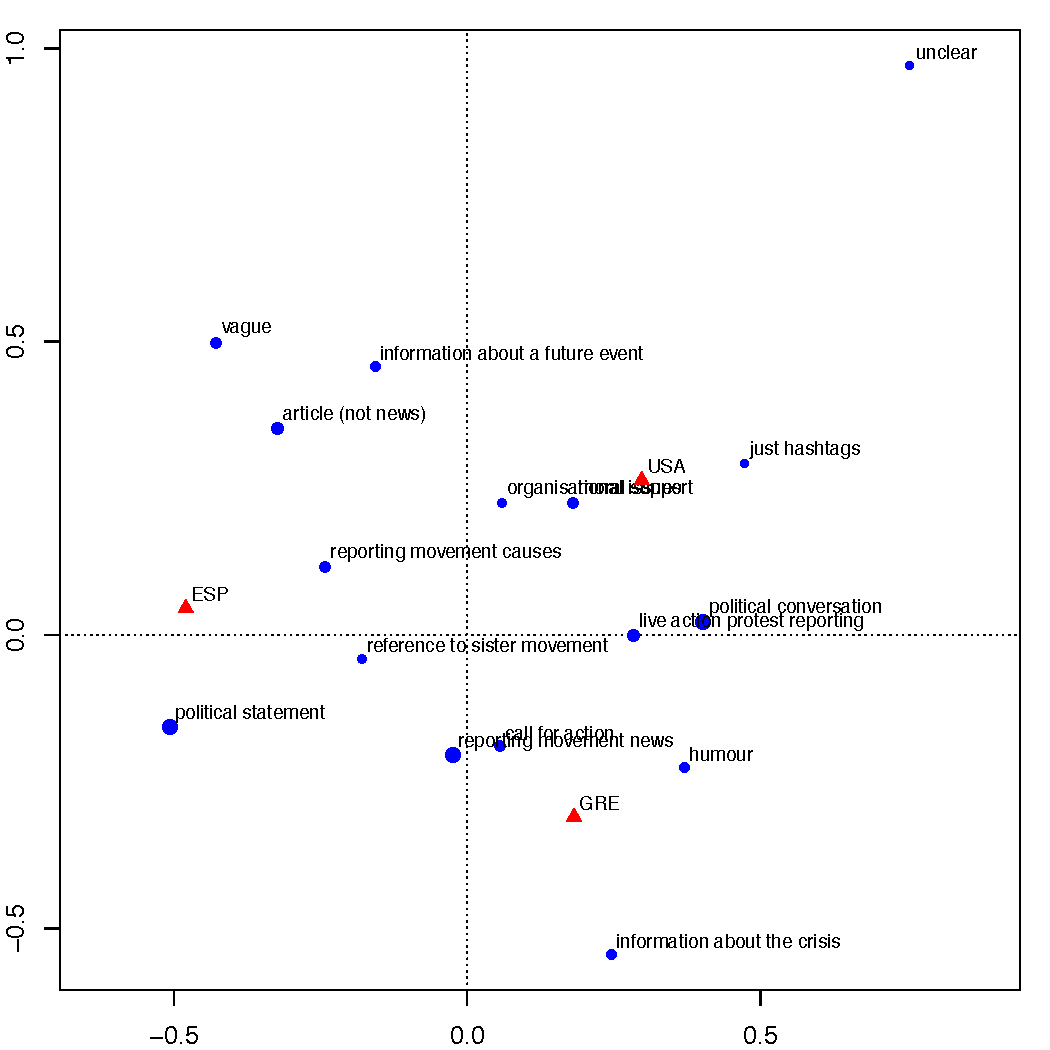
\includegraphics[scale=1]{purpose-by-country-ca2}}
\centerline{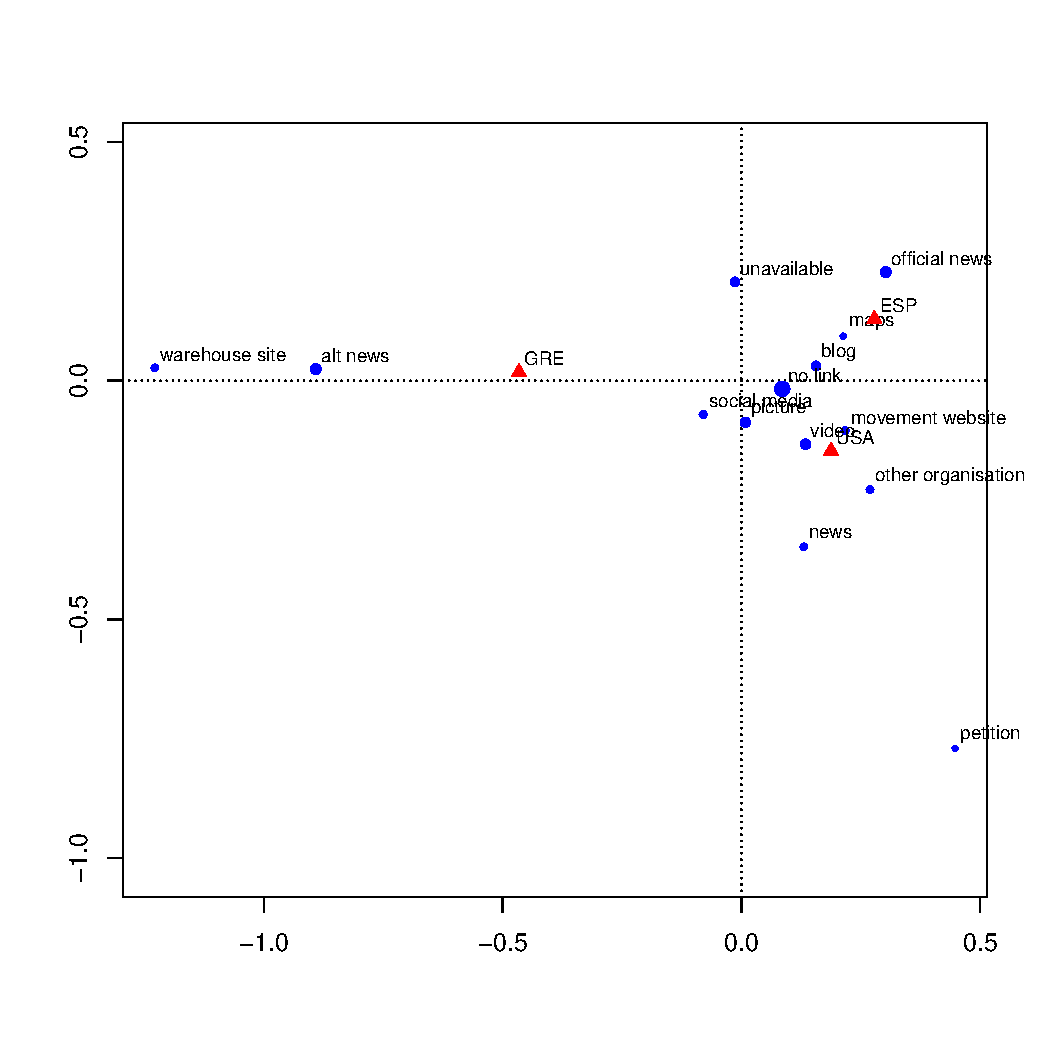
\includegraphics[scale=1]{linktarget-by-country-ca}}
\centerline{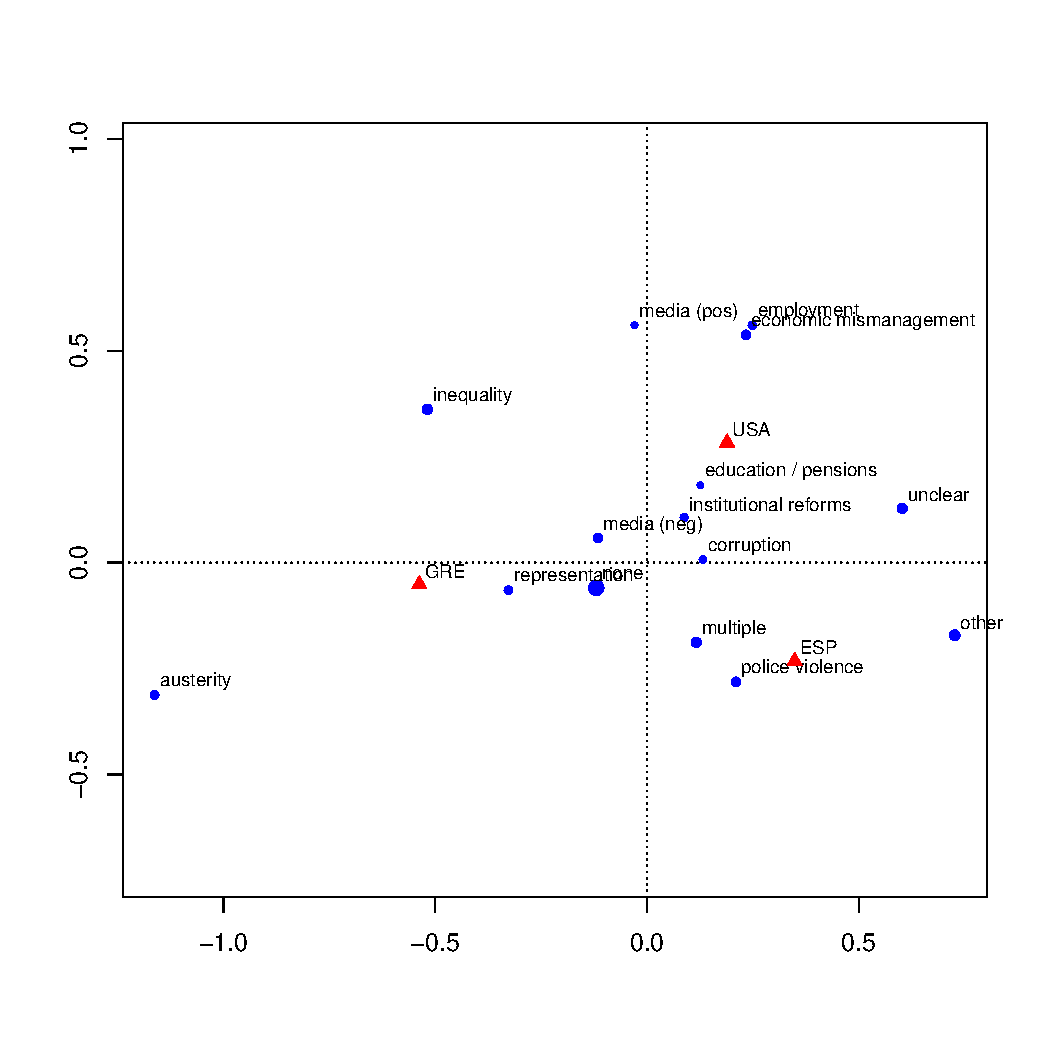
\includegraphics[scale=1]{issues-by-country-ca}}

%\slide{}
%
%
%\slide{A surprising application to IR}
%                                                      
%Russian artillery south of the Chechen
%capital Grozny blasted Chechen
%positions overnight before falling silent
%at dawn, witnesses said on Tuesday.
%
%\noindent                                                                       
%Israel said on Tuesday it sent
%  humanitarian aid to
%Colombia where a massive
%  earthquake last week
%killed at least 938 people and injured 400.
%
%\slide{Event data extraction}
%
%                                                                                                                               
%\mkred{Russian artillery}$^{\,\mathsf{S}}$ south of the Chechen
%capital
%Grozny \mkgreen{blasted}$^{\,\mathsf{223}}$ \mkblue{Chechen
%positions}$^{\,\mathsf{T}}$ overnight before falling silent
%at dawn, witnesses said on Tuesday.
%
%\noindent                                                          
%\mkred{Israel}$^{\,\mathsf{S}}$ said on Tuesday it \mkgreen{sent
%  humanitarian aid}$^{\,\mathsf{073}}$ to
%\mkblue{Colombia}$^{\,\mathsf{T}}$ where a \mkred{massive
%  earthquake}$^{\,\mathsf{S}}$ last week
%\mkgreen{killed}$^{\,\mathsf{222}}$ at least \mkblue{938~
%people}$^{\,\mathsf{T}}$ and injured 400.
%~\\
%
%\slide{Event data extraction}
%
%                                                                                                                               
%\mkred{Russian artillery}$^{\,\mathsf{S}}$ south of the Chechen
%capital
%Grozny \mkgreen{blasted}$^{\,\mathsf{223}}$ \mkblue{Chechen
%positions}$^{\,\mathsf{T}}$ overnight before falling silent
%at dawn, witnesses said on Tuesday.
%
%\noindent                                                          
%\mkred{Israel}$^{\,\mathsf{S}}$ said on Tuesday it \mkgreen{sent
%  humanitarian aid}$^{\,\mathsf{073}}$ to
%\mkblue{Colombia}$^{\,\mathsf{T}}$ where a \mkred{massive
%  earthquake}$^{\,\mathsf{S}}$ last week
%\mkgreen{killed}$^{\,\mathsf{222}}$ at least \mkblue{938~
%people}$^{\,\mathsf{T}}$ and injured 400.
%~\\
%{\large
%\begin{center}
%\texttt{20010901 RUS CHE 223}\\
%\texttt{20020804 ISR COL 073}\\
%\texttt{20020804 --- COL 222}
%\end{center}
%}
%\slide{Dyadic event data (Serbia-Bosnia)}
%
%\begin{center} 
%{\footnotesize
%\begin{tabular}{rrr} \toprule
%Week       & Code & Description \\ \midrule
%1995-07-11 & 211 & SEIZE POSSESSION \\
% & 212 & ARREST PERSON \\
% & 223 & MILITARY ENGAGEMENT \\ \midrule
%1995-07-12 & 211 & SEIZE POSSESSION \\
% & 223 & MILITARY ENGAGEMENT \\
% & 173 & SPECIF THREAT \\
% & 191 & CANCEL EVENT \\
% & 211 & SEIZE POSSESSION \\
% & 095 & PLEAD \\
% & 111 & TURN DOWN \\
% & 212 & ARREST PERSON \\
% & 081 & MAKE AGREEMENT \\
% & 023 & NEUTRAL COMMENT \\
% & 032 & VISIT \\
% & 031 & MEET \\ \bottomrule
%\end{tabular}
%}
%\end{center}
%
%\newpage
%
%\slide{Scaled dyadic event data}
%
%\begin{center} 
%{\footnotesize
%\begin{tabular}{rrr} \toprule
%Week       & Code & Score [-10,10) \\ \midrule
%1995-07-11 & 211 & -9.2 \\
% & 212 & -9.0 \\
% & 223 & -10.0 \\ \midrule
%1995-07-12 & 211 & -9.2 \\
% & 223 & -10.0 \\
% & 173 & -7.0 \\
% & 191 & -2.2 \\
% & 211 & -9.2 \\
% & 095 & 1.2 \\
% & 111 & -4.0  \\
% & 212 & -9.0 \\
% & 081 & 6.5 \\
% & 023 & -0.2 \\
% & 032 & 1.9 \\
% & 031 & 1.0 \\ \bottomrule
%\end{tabular}
%}
%\end{center}
%
%\slide{Summed scaled dyadic event data}
%
%\centerline{\includegraphics[scale=.8]{fatsum}}
%
%\slide{The human elements}
%
%\textit{Coders} read newswire and extract events\\ \mkgrey{(e.g. GEDS projects, Swisspeace)}
%
%\textit{Experts} assign scores to event types\\
%\mkgrey{(e.g. Goldstein 1995, Shellman 2004)}
%
%\textit{Analysts} aggregate and infer conflict dynamics\\ \mkgrey{(Goldstein \& Pevehouse 1997, Pevehouse \& Goldstein 1999)}
%
%\slide{Automating a conflict scale}
%
%Schrodt (2007) applied IRT models to event data
%
%Motivation: 
%\ita
%\itm International actions in a week are like roll-call votes in a parliament 
%\itm or like responses on a survey (with lots of questions) 
%\itz 
%\pause 
%But it didn't work
%\pause
%There's a \textit{substantive} reason for that
%
%\slide{Two kinds of item structure}
%
%\textbf{Dominance}
%
%IRT models used in voting, surveying, and testing applications assume that \textit{perfect data} would have dominance structure
%
%~\\
%\centerline{\small
%\begin{tabular}{rcccccccc} 
%& \multicolumn{3}{l}{`easy'} & & & \multicolumn{3}{r}{`hard'}\\
%\toprule
%&A & B & C & D & E & F & G & H \\ \midrule
%low $\theta$&1 & 1 & 1 & 0 & 0 & 0 & 0 & 0 \\
%&1 & 1 & 1 & 1 & 0 & 0 & 0 & 0 \\
%&1 & 1 & 1 & 1 & 1 & 0 & 0 & 0 \\
%&1 & 1 & 1 & 1 & 1 & 1 & 0 & 0 \\
%&1 & 1 & 1 & 1 & 1 & 1 & 1 & 0 \\
%high $\theta$&1 & 1 & 1 & 1 & 1 & 1 & 1 & 1 \\
%\bottomrule
%\end{tabular}
%}
%
%\slide{Two kinds of item structure}
%
%\textbf{Proximity}
%
%Unfolding models used in ideal point estimation assume that \textit{perfect data} would have a structure
%
%~\\
%\centerline{\small
%\begin{tabular}{rcccccccc} \toprule
%& \multicolumn{3}{l}{`left'} & & & \multicolumn{3}{r}{`right'}\\
%& A & B & C & D & E & F & G & H \\ \midrule
%`left' $\theta$&1 & 1 & 1 & 0 & 0 & 0 & 0 & 0 \\
%&0 & 1 & 1 & 1 & 0 & 0 & 0 & 0 \\
%&0 & 0 & 1 & 1 & 1 & 0 & 0 & 0 \\
%&0 & 0 & 0 & 1 & 1 & 1 & 0 & 0 \\
%&0 & 0 & 0 & 0 & 1 & 1 & 1 & 0 \\
%`right' $\theta$&0 & 0 & 0 & 0 & 0 & 1 & 1 & 1\\
%\bottomrule
%\end{tabular}
%}
%
%\slide{Unfolding models for event data}
%
%Happily we have \textit{several}, often used for text scaling:
%
%{\large
%\begin{align*}
%\text{log}\, E[Y_{ij}] &= \alpha_i + \psi_j + 
%{\color{bloodred}\theta_i}\,{\color{darkblue}\beta_j} & \text{RC Model}\\
%~\\
%Y_{ij}/N &= \alpha_i\, \psi_j\, (1 + 
%{\color{bloodred}\theta_i}\,{\color{darkblue}\beta_j}) & \text{CA}
%\end{align*}
%}
%
%$Y_i$ is a table each week's events counts (a `document')\\
%Scale weeks ${\color{bloodred}\theta_i}$ and infer event types ${\color{darkblue}\beta_j}$
%
%
%\slide{First example}
%
%\textbf{Scaling CAMEO codes in the Middle East (ISR-PAL)}
%
%Aggregate event types up to 20 top level CAMEO categories
%
%Compare to weekly averaged Goldstein scores (1979-2011)
%
%\slide{Manual vs induced weekly conflict $\theta$}
%
%\centerline{\includegraphics[scale=1]{cameo-weeks}}
%\centerline{$r=0.89$}
%
%\slide{Item scores $\beta$ for event types}
%
%\begin{center}
%\includegraphics[scale=1]{cameo-items}
%\end{center}
%
%\slide{Did we need all those categories?}
%
%\textbf{Scaling WEIS codes in Yugoslavia (SER-BOS)}
%
%Aggregate to 4 basic event categories \mkgrey{(Schrodt, 2012)}
%
%{\footnotesize
%\begin{center}
%\begin{tabular}{lrrrrr} \toprule
%Week & Mat.Conf. & Mat.Coop. & Verb.Conf. & Verb.Coop. & ~~~~~$N_t$ \\ \midrule
%~~~\vdots &  \vdots~ & \vdots~ & \vdots~ & \vdots~ &  \vdots\\
%1995-07-09  &     29   &     3  &      4  &      5  & 41\\
%1995-07-16  &     21   &     4  &     12  &     13  & 50\\
%1995-07-23  &     12   &     3  &      4  &      1  & 20 \\
%1995-07-30  &      4   &     2  &      2  &      4  & 12\\ 
%~~~\vdots &  \vdots~ & \vdots~ & \vdots~ & \vdots~ & \vdots~\\ \midrule 
%            &      939 &  380  &    304  &    483 &  \\
%\bottomrule
%\end{tabular}
%\end{center}
%}
%
%~\\
%Compare to weekly averaged Goldstein scores
%
%\slide{Manual vs induced weekly conflict $\theta$}
%
%\begin{center}
%\includegraphics[scale=.8]{errors-rc}
%\includegraphics[scale=.8]{errors-ca}
%\end{center}
%\centerline{~~~$r$=0.84 ~~~~~~~~~~~~~~~~~ $r$=0.9}
%
%\slide{Item scores $\beta$ for event types}
%
%This works because both models recover the type-averaged Goldstein scores
%
%~\\
%{\small
%\begin{center}
%\begin{tabular}{lrrr}
%  \toprule
%Event & Av. Goldstein & RC & CA \\ 
%  \midrule
%material conflict    & -1.13 &  -1.42 &   -1.27 \\ 
%verbal conflict      & -0.54 &   0.02  &  -0.28 \\ 
%verbal cooperation   &  0.72  &  0.60  &   0.55 \\ 
%material cooperation &  0.95  &  0.80  &   1.00 \\  \midrule
%                     &        &  $r$=0.93 & $r$=0.98 \\
%\bottomrule
%\end{tabular}
%\end{center}
%}
%
%\slide{Item scores for event types}
%
%\begin{center}
%\includegraphics[scale=.9]{newbiplot}
%\end{center}
%
%
%
%\slide{Automating a conflict scale}
%
%Those event coders and conflict experts were onto something\ldots
%\ita
%\itm and we understand it enough to automate it
%\itz
%\pause
%Substantively
%\ita
%\itm expert-validated event scaling is now cheap and potentially important for bringing \textit{context sensitivity} back into event data analysis
%\itz
%
\slide{In conclusion}

\centerline{What are you going to scale today?}

\slide{In grander conclusion}

If you ask for topics, you'll get topics

If you ask for classifications, you'll get classifications

If you ask for positions, you'll get positions

\ldots

Ask for what makes sense\ldots

\slide{}

\slide{CA as an (approximation to) unfolding}

An unfolding type `unimodal model' \mkgrey{(ter Braak 1985)}

~\\
\centerline{\includegraphics[scale=1]{ter-braak-unimodal-model}}

CA transition eqns. \hfill ML unimodal model update eqns.

~\\
\centerline{\includegraphics[scale=1]{ter-braak-transition-equations}
\includegraphics[scale=1]{ter-braak-ca-approximation-unimodal-model}}

see also \mkgrey{(Heiser 1981, Polak et al. 2009)}


\end{document}
